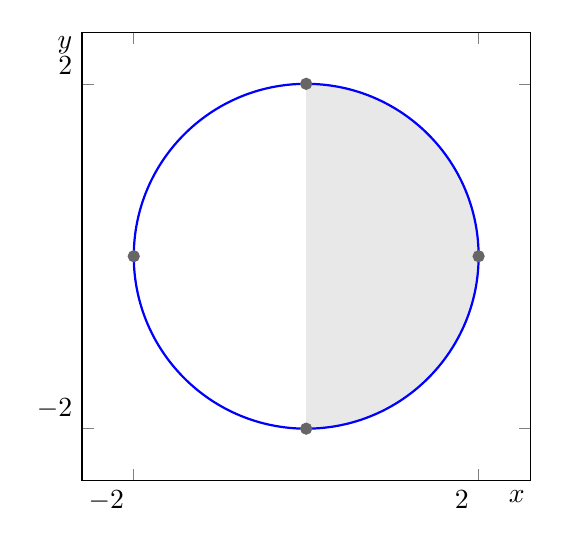
\begin{tikzpicture}[scale=1]

% === Parâmetros ===
\def\r{2}   % raio do círculo

  \begin{axis}[      
      xlabel={$x$}, ylabel={$y$},
      axis equal image,        % mantém escala x=y para o círculo não ficar ovalado
      xmin=-1.3*\r, xmax=1.3*\r, ymin=-1.3*\r, ymax=1.3*\r,
      xtick={-\r,\r}, ytick={-\r,\r},
      x tick label style={anchor=north east}, % rótulos abaixo e a esquerda do eixo X
      y tick label style={anchor=south east}, % rótulos acima e a esquerda do eixo y
      % width=8cm, height=6cm,
      every axis x label/.style={at={(ticklabel* cs:0.97)}, anchor=north},
      every axis y label/.style={at={(ticklabel* cs:0.97)}, anchor=east},
    ]

    % --- Região sombreada: metade direita do círculo ---
    \path[fill=gray!30, opacity=0.6]
      (axis cs:0,-\r)     % Ponto inicial, no eixo y
      arc[start angle=-90, end angle=90, radius=\r] % Arco da metade direita
      -- cycle;           % Fecha com o diâmetro vertical

    % --- Curvas ---
    \draw[thick, blue] (axis cs:0,0) circle [radius=\r];    % Círculo de raio r

    % --- Pontos de interseção com os eixos ---
    \addplot[only marks, black!60, mark=*] coordinates {(\r,0) (-\r,0) (0,\r) (0,-\r)};


  \end{axis}
  
\end{tikzpicture}
